\subsection{题目描述}
\noindent One-dimensional Kronig-Penney problem. Considering the Hamiltonian of the system as 
\[
\hat{H} = -\frac{\hbar^2}{2 m_e} \frac{\partial^2}{\partial x^2} + V(x)
\]
with a one-dimensional periodic potential \( V(x) = V(x + a) \). The potential can be expressed as 
\[
V(x) = 
\begin{cases}
0, & \text{if } 0  \leq x < L_W, \\
U_0, & \text{if } L_W \leq x < a
\end{cases}
\]
and the period of the potential is $a = L_W+L_B$, which is also shown in the Figure below.

\begin{figure}[H]
    \centering
    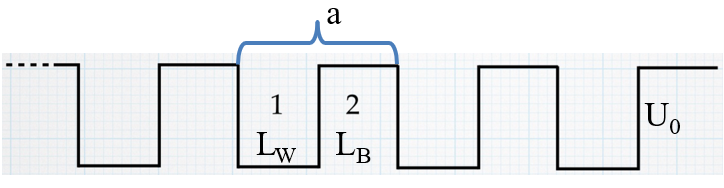
\includegraphics[width=1.0\textwidth]{Problem_1/figs/potential_well.png}
    \caption{Kronig-Penney potential well}
\end{figure}
\noindent With parameters:
\[
U_0 = 2 \, \text{eV}, \quad L_W = 0.9 \, \text{nm}, \quad L_B = 0.1 \, \text{nm} \quad (a = 1 \, \text{nm})
\]
Using FFT, find the lowest three eigenvalues of the electric eigenstates that satisfy 
\[
\hat{H} \psi_i = E \psi_i \quad \text{and} \quad \psi_i(x) = \psi_i(x + a).
\]
Explanation: Since the system is translation-invariant, i.e., \( \psi_i(x) = \psi_i(x + a) \), we can use the plane wave basis expansion 
$$ \psi(x) = \frac{1}{\sqrt{a}} \sum_q C_q e^{i q \frac{2\pi}{a} x} ,\quad q = -N, -N + 1, \dots, -1, 0, 1, \dots, N - 1, N .$$

\noindent In this basis set, the Hamiltonian can be represented in matrix form as
\[H_{pq}=\frac{1}{a}\langle e^{ip\frac{2\pi}{a}x}|\hat{H}|e^{iq\frac{2\pi}{a}x}\rangle_{\mathrm{cell}}=\frac{1}{a}\int_{0}^{a}dx e^{-ip\frac{2\pi}{a}x}\hat{H}e^{iq\frac{2\pi}{a}x}.\]
To calculate \( \hat{H} e^{i q \frac{2\pi}{a} x} \), the periodic potential \( V(x) \) can be expanded in Fourier series as \( V(x) \rightarrow V_q \), where 
\[ V(x) = \sum_{q'=-N}^{N} V_{q'} e^{i q' \frac{2\pi}{a} x} .\]
The basis wave function can then be written as:
\[\hat{H}e^{iq\frac{2\pi}{a}x}=(\hat{T}+\hat{V})e^{iq\frac{2\pi}{a}x}=\frac{2\hbar^2q^2\pi^2}{ma^2}e^{iq\frac{2\pi}{a}x}+\sum_{q^{\prime}=-N}^NV_{q^{\prime}}e^{i(q^{\prime}+q)\frac{2\pi}{a}x}\]
Try constructing the Hamiltonian matrix \( H_{pq} \) and solve the eigenvalue equation \( \hat{H} \psi_i = E \psi_i \) to obtain the three lowest energy eigenvalues.

\noindent \textit{Special note:} You can use built-in functions to simplify the eigenvalue calculations and FFT transformations.


\subsection{程序描述}

\subsection{伪代码}
Powered by \href{https://chatgpt.com/g/g-xJJAA2awf-latex-pseudocode-generator}{\LaTeX \ pseudocode generator}

\subsection{结果示例}

